\documentclass{article}
\usepackage[utf8]{inputenc}
\usepackage[spanish]{babel}
\usepackage{graphicx}
\usepackage{hyperref}
\usepackage{amsmath}
\usepackage{geometry}
\usepackage{booktabs}
\usepackage{adjustbox}
\usepackage{caption}
\usepackage{multirow}
\usepackage{pdflscape}
\usepackage{float}
\usepackage{array}
\geometry{a4paper, margin=1in}

\hypersetup{
    colorlinks=true,
    linkcolor=black,
    urlcolor=blue,
    citecolor=black
}

\title{Solución iterativa de Jacobi para la ecuación de Poisson 1D\\[0.5em]
\large Reto 1 --- Computación de Alto Rendimiento}
\author{Daniel Toro Soto - Juan Camilo Galvis}
\date{Marzo 2026}

\begin{document}

\maketitle


\begin{abstract}
El presente documento describe la implementación y análisis comparativo del
método iterativo de Jacobi aplicado a la ecuación de Poisson 1D con condiciones
de frontera de Dirichlet, evaluado bajo cinco estrategias de ejecución:
secuencial sin optimizaciones, secuencial con \texttt{-O2}, secuencial con
optimización de acceso a memoria (fusión de lazos y swap de punteros), paralelo
mediante hilos POSIX (\texttt{pthread}) y paralelo mediante procesos
(\texttt{fork}).  Las pruebas se realizaron sobre mallas de $N = 2^k + 1$ nodos
con $k \in \{1,\ldots,11\}$ (es decir, desde $N=3$ hasta $N=2\,049$) con 10
repeticiones por configuración para las variantes secuenciales e hilos; las
variantes de multiprocesamiento se ejecutaron con una sola repetición debido al
alto costo computacional.  Los experimentos se llevaron a cabo en un ASUS~TUF
Gaming con procesador Intel Core~i5-10300H (4 núcleos físicos, 8 hilos lógicos),
16~GB de RAM y sistema operativo Kali~Linux (kernel~6.x, GNOME) bajo carga de
corriente continua.  Se analizan tiempos de ejecución en reloj de pared,
\emph{speedup} respecto al secuencial base y el impacto de la barrera de
sincronización en el rendimiento paralelo.
\end{abstract}


\newpage
\tableofcontents
\newpage

% ─────────────────────────────────────────────────────────────────────────────
\section{Introducción}

La ecuación de Poisson 1D es uno de los problemas de referencia en cómputo
científico: sencilla de formular pero representativa de la clase de sistemas
lineales densos que emergen de la discretización de ecuaciones en derivadas
parciales.  Su solución iterativa mediante el método de Jacobi exhibe una
convergencia lenta ($\mathcal{O}(h^2)$ por iteración, con $h=1/(N-1)$ el paso
de malla) que la convierte en un candidato ideal para cuantificar el impacto de
las optimizaciones de compilador, la localidad de caché y las estrategias de
paralelismo.

En este reto se implementaron cinco variantes del solucionador en C, siguiendo
la formulación de Burkardt~\cite{burkardt}, y se midieron sus tiempos de
ejecución en reloj de pared sobre un equipo de gama media con un procesador
Intel de cuatro núcleos.  El objetivo es determinar qué estrategia ofrece la
mejor relación costo-rendimiento para resolver la ecuación de Poisson 1D y
comprender por qué el paralelismo puede ser contraproducente cuando el trabajo
útil por iteración es demasiado pequeño frente al costo de sincronización.

% ─────────────────────────────────────────────────────────────────────────────
\section{Marco Conceptual}

\subsection{High Performance Computing (HPC)}

La Computación de Alto Rendimiento (HPC) agrupa técnicas y arquitecturas
diseñadas para resolver problemas con altos requisitos computacionales en el
menor tiempo posible.  Cuando hablamos de HPC, ``hacemos referencia a un campo
de la computación actual que da solución a problemas tecnológicos muy complejos
y que involucran un gran volumen de cálculos o de coste computacional''
(López, 2017).  En este reto, el número de iteraciones de Jacobi crece
aproximadamente como $\mathcal{O}(N^2)$, lo que hace que el problema sea
sensible al tamaño de la malla y justifica la exploración de estrategias de
paralelización y optimización.

\subsection{Ecuación de Poisson 1D y discretización}

Se resuelve el problema de valor en la frontera:
\[
  u''(x) = f(x), \quad x \in (0,1), \qquad u(0) = u(1) = 0,
\]
con función forzante $f(x) = -x(x+3)e^x$, cuya solución exacta es
$u(x) = x(x-1)e^x$.

La discretización de diferencias finitas centradas con paso $h = 1/(N-1)$
conduce al sistema lineal tridiagonal $Au = \mathbf{f}$, donde los elementos de
$A$ son $A_{ii} = 2/h^2$ y $A_{i,i\pm 1} = -1/h^2$~\cite{burkardt}.

\subsection{Método iterativo de Jacobi}

El método de Jacobi actualiza simultáneamente todos los nodos interiores en cada
barrido:
\[
  u_j^{(k+1)} = \frac{f_j h^2 + u_{j-1}^{(k)} + u_{j+1}^{(k)}}{2},
  \quad j = 1, \ldots, N-2.
\]
La convergencia se verifica en términos del residuo cuadrático medio (RMS):
\[
  \text{RMS} = \sqrt{\frac{1}{N}\sum_{j=0}^{N-1} r_j^2},
\quad
  r_j = (Au^{(k)})_j - f_j,
\]
deteniéndose cuando $\text{RMS} \leq \varepsilon = 10^{-6}$.  El número de
iteraciones necesarias crece aproximadamente como $\mathcal{O}(N^2)$, por lo que
para $k=11$ ($N=2\,049$) se requieren más de 12 millones de
barridos~\cite{burkardt}.

\subsection{Localidad de caché y optimización de acceso}

Para mallas pequeñas a medianas, el costo dominante no es la aritmética sino el
movimiento de datos entre CPU y memoria.  La variante \texttt{JacobiMemory}
aplica cuatro optimizaciones: (1)~fusión del lazo de barrido y el cómputo del
residuo en un solo recorrido del vector; (2)~\emph{swap} de punteros en lugar de
copiar el arreglo entre iteraciones; (3)~verificación infrecuente de la
convergencia (cada 50 iteraciones) para reducir las operaciones de punto flotante
en la comprobación; y (4)~uso de aritmética de punteros para mejorar el acceso
secuencial en caché.

\subsection{Programación paralela}

La ``computación paralela es el uso de múltiples recursos computacionales para
resolver un problema, en la que varias operaciones pueden ocurrir
simultáneamente'' (Ferestrepoca, 2019).  En este proyecto se emplean dos
mecanismos:

\begin{itemize}
  \item \textbf{Hilos POSIX (\texttt{pthread})}: comparten el espacio de memoria
    del proceso.  Cada hilo procesa un segmento del vector $u$; al final de cada
    barrido, todos sincronizan con \texttt{pthread\_barrier\_wait} antes del
    siguiente.
  \item \textbf{Procesos (\texttt{fork})}: cada proceso tiene su propio espacio
    de memoria; el vector resultado se aloja en memoria compartida anónima
    (\texttt{mmap(MAP\_SHARED|MAP\_ANONYMOUS)}) y las matrices de entrada se
    heredan por semántica \emph{copy-on-write}.
\end{itemize}

\subsection{Hilos vs.\ Procesos}

La diferencia fundamental es que ``un proceso dispone de un espacio de memoria
separado, mientras que un hilo no. De esta forma los hilos pueden trabajar
directamente con las variables creadas por el proceso padre, mientras que los
procesos hijos no pueden hacerlo'' (Montero \& Antunez, 2011).  Para el método
de Jacobi 1D, esta diferencia se traduce en que los hilos pueden leer
directamente los valores del vector vecino sin copias intermedias, mientras que
los procesos deben usar la región de memoria compartida, introduciendo latencias
adicionales.

\subsection{Speedup y Ley de Amdahl}

El speedup mide la ganancia de rendimiento de la versión paralela:
\[
  S_p = \frac{T^*(N)}{T_p(N)},
\]
donde $T^*(N)$ es el tiempo secuencial de referencia y $T_p(N)$ el tiempo
con $p$ trabajadores.  El speedup ideal es $S_p = p$, pero la Ley de
Amdahl~\cite{amdahl} establece que la fracción serial del algoritmo impone un
límite superior.  En el caso del método de Jacobi con barreras de
sincronización, el \emph{overhead} de cada \texttt{pthread\_barrier\_wait} es la
fracción serial dominante; con millones de iteraciones, ese costo supera
ampliamente el trabajo útil para mallas pequeñas.

% ─────────────────────────────────────────────────────────────────────────────
\section{Marco Contextual}

\subsection{Características de la máquina}

Las pruebas se realizaron sobre el siguiente hardware:

\begin{itemize}
  \item \textbf{Equipo:} ASUS TUF Gaming (2020)
  \item \textbf{Procesador:} Intel Core i5-10300H --- 4 núcleos físicos / 8
    hilos lógicos (Hyper-Threading), base 2.5~GHz, turbo 4.5~GHz, 8~MB caché
    L3, proceso 14~nm
  \item \textbf{GPU:} NVIDIA GeForce GTX~1650 (no utilizada en los benchmarks)
  \item \textbf{Memoria:} 16~GB RAM DDR4
  \item \textbf{Almacenamiento:} 512~GB SSD NVMe
  \item \textbf{Sistema operativo:} Kali Linux (entorno gráfico GNOME), siempre
    conectado a la corriente
  \item \textbf{Compilador:} GCC (versión de sistema Kali)
\end{itemize}

El i5-10300H cuenta con 4 núcleos físicos y 8 hilos lógicos gracias a
Hyper-Threading.  Para configuraciones de 8 hilos o más, varios hilos comparten
un mismo núcleo físico, lo que puede agravar la contención en la caché L1/L2
privada y amplificar el efecto negativo de las barreras de sincronización.

Las pruebas evaluaron mallas de índice $k \in \{1, 2, 3, 4, 5, 6, 7, 8, 9, 10, 11\}$, correspondientes a $N = 2^k + 1$ nodos interiores:
$N \in \{3, 5, 9, 17, 33, 65, 129, 257, 513, 1025, 2049\}$,
con \textbf{10 repeticiones} por configuración para las variantes secuenciales e
hilos.  Las variantes de multiprocesamiento se ejecutaron con \textbf{una sola
repetición} por su elevado costo (la variante de 16 procesos solo pudo completar
hasta $k=8$ antes de que el tiempo de ejecución se volviese excesivo).

\subsection{Desarrollo}

Las cinco implementaciones en C comparten la misma estructura base: inicialización del vector solución a cero, evaluación de la función forzante, iteraciones de Jacobi y medición del tiempo de reloj de pared mediante \texttt{clock\_gettime(CLOCK\_MONOTONIC)}.  El tiempo impreso en \texttt{stdout} corresponde al tiempo transcurrido en segundos con 6 decimales, seguido del número de iteraciones realizadas.

\begin{description}
  \item[\texttt{secuential}] Jacobi ingenuo: copia $u \to u\_old$ en cada
    barrido, actualiza todos los nodos interiores y verifica el RMS en cada
    iteración.  Compilado sin optimizaciones (\texttt{-O0} implícito).
  \item[\texttt{secuentialFlags}] Mismo código fuente que \texttt{secuential},
    compilado con \texttt{-O2} para medir el impacto de las optimizaciones
    automáticas del compilador (vectorización automática, reordenamiento de
    instrucciones, etc.).
  \item[\texttt{memory}] Cuatro optimizaciones manuales: fusión del lazo de
    barrido y residuo, swap de punteros, verificación de convergencia cada 50
    iteraciones y aritmética de punteros.  Compilado sin \texttt{-O2}.
  \item[\texttt{threads}] Divide los nodos interiores entre $p$ hilos POSIX;
    cada hilo actualiza su segmento y luego espera en
    \texttt{pthread\_barrier\_wait} antes del siguiente barrido.  El hilo 0
    verifica el RMS tras la barrera.
  \item[\texttt{multiprocessing}] Crea $p$ procesos hijo con \texttt{fork()};
    el vector $u$ reside en memoria compartida anónima.  Cada proceso actualiza
    su segmento; la coordinación entre iteraciones se realiza a través del
    vector compartido sin barrera explícita, con el proceso padre verificando la
    convergencia.
\end{description}

\subsection{Sistema de compilación (Makefile)}

El proyecto utiliza un \texttt{Makefile} que compila los cinco binarios en el directorio \texttt{output/}:

\begin{verbatim}
make              # Compila los 5 binarios
make clean        # Elimina output/
\end{verbatim}

Todos los binarios usan las banderas \texttt{-Wall -lm}.  La variante
\texttt{secuentialFlags} agrega \texttt{-O2}; la variante \texttt{threads}
agrega \texttt{-pthread}.

\subsection{Estrategia de benchmarking}

El script \texttt{scripts/RunAll.sh} implementa un sistema de reanudación
automática basado en \emph{checkpoints}: cada medición exitosa se registra en
\texttt{checkpoint.log} con la clave \texttt{<tipo>,<k>,<config>,<run>}, y las
ejecuciones ya completadas se omiten en reinicios posteriores.  Al finalizar, el
directorio de resultados recibe el sufijo \texttt{.done}.

Para el multiprocesamiento se utilizó el script auxiliar
\texttt{scripts/RunMultiprocessingQuick.sh}, que realiza una sola repetición por
configuración dada la duración excesiva de las corridas completas.  La
configuración de 16 procesos se interrumpió manualmente al llegar a $k=8$ ($N=257$), ya que la ejecución de $k=9$ y superiores resultaba impráctica.

\subsection{Medición de tiempo de reloj de pared}

A diferencia de herramientas que miden tiempo de CPU acumulado
(\texttt{getrusage}), todas las implementaciones de este reto usan
\texttt{clock\_gettime(CLOCK\_MONOTONIC)} para medir el tiempo real transcurrido:

\begin{verbatim}
struct timespec start, end;
clock_gettime(CLOCK_MONOTONIC, &start);
/* ... iteraciones de Jacobi ... */
clock_gettime(CLOCK_MONOTONIC, &end);
double elapsed = (end.tv_sec  - start.tv_sec)
               + (end.tv_nsec - start.tv_nsec) / 1e9;
\end{verbatim}

\texttt{CLOCK\_MONOTONIC} garantiza que el tiempo nunca retrocede (robusto frente
a ajustes del reloj del sistema) y reporta el tiempo de pared independientemente
del número de hilos o procesos activos.  Esto permite comparar directamente
todas las variantes: si la versión con 2 hilos tarda 236~s y la secuencial
tarda 205~s, esos son los segundos reales que el usuario espera, y el speedup
es $205/236 < 1$ (la versión paralela es más lenta).

% ─────────────────────────────────────────────────────────────────────────────
\section{Pruebas}

A continuación se presentan los tiempos de ejecución en segundos (sobre 10
repeticiones para variantes secuenciales e hilos; 1 repetición para
multiprocesamiento) para cada implementación.  Las columnas corresponden a los
índices de malla $k=1,\ldots,11$ ($N = 2^k+1$ nodos).  La fila
\textbf{Pr} indica el promedio de las 10 corridas; la fila
\textbf{Speedup} indica el cociente $T_{\text{sec}} / T_{\text{var}}$ calculado
sobre los promedios (valores $<1$ indican \emph{mayor} tiempo que el secuencial).

\subsection{Secuencial}

\begin{table}[H]
\centering
\tiny
\begin{tabular}{|c|c|c|c|c|c|c|c|c|c|c|c|}
\hline
\multicolumn{12}{|c|}{\textbf{Secuencial (sin optimizaciones)}} \\
\hline
\textbf{Ejec.} & \textbf{k=1} & \textbf{k=2} & \textbf{k=3} & \textbf{k=4} & \textbf{k=5} & \textbf{k=6} & \textbf{k=7} & \textbf{k=8} & \textbf{k=9} & \textbf{k=10} & \textbf{k=11} \\
\textbf{} & \textbf{N=3} & \textbf{N=5} & \textbf{N=9} & \textbf{N=17} & \textbf{N=33} & \textbf{N=65} & \textbf{N=129} & \textbf{N=257} & \textbf{N=513} & \textbf{N=1025} & \textbf{N=2049} \\
\hline
1  & 0.000020 & 0.000032 & 0.000060 & 0.000155 & 0.001124 & 0.008008 & 0.056247 & 0.397168 & 3.360862 & 25.664168 & 204.892441 \\
2  & 0.000012 & 0.000013 & 0.000025 & 0.000117 & 0.000802 & 0.006258 & 0.051009 & 0.393642 & 3.299488 & 25.543362 & 204.583612 \\
3  & 0.000011 & 0.000012 & 0.000026 & 0.000121 & 0.000810 & 0.006408 & 0.050487 & 0.391746 & 3.243976 & 25.872457 & 204.865405 \\
4  & 0.000011 & 0.000013 & 0.000025 & 0.000115 & 0.000823 & 0.006200 & 0.050210 & 0.392225 & 3.302961 & 25.504304 & 204.758206 \\
5  & 0.000012 & 0.000013 & 0.000026 & 0.000123 & 0.000820 & 0.006317 & 0.051001 & 0.398548 & 3.236667 & 26.365962 & 204.972648 \\
6  & 0.000012 & 0.000013 & 0.000024 & 0.000115 & 0.000804 & 0.006483 & 0.054709 & 0.446152 & 3.392824 & 25.729952 & 205.007244 \\
7  & 0.000012 & 0.000012 & 0.000030 & 0.000120 & 0.000842 & 0.006296 & 0.049824 & 0.439149 & 3.422229 & 25.646188 & 209.518479 \\
8  & 0.000013 & 0.000013 & 0.000025 & 0.000114 & 0.000842 & 0.006444 & 0.050546 & 0.413830 & 3.423978 & 25.685489 & 206.677936 \\
9  & 0.000012 & 0.000013 & 0.000025 & 0.000115 & 0.000860 & 0.006387 & 0.050338 & 0.410801 & 3.380627 & 25.661951 & 204.967757 \\
10 & 0.000012 & 0.000013 & 0.000025 & 0.000117 & 0.000801 & 0.006318 & 0.050798 & 0.418120 & 3.416599 & 25.731771 & 205.487066 \\
\hline
\textbf{Pr} & \textbf{0.000013} & \textbf{0.000015} & \textbf{0.000029} & \textbf{0.000121} & \textbf{0.000853} & \textbf{0.006512} & \textbf{0.051517} & \textbf{0.410138} & \textbf{3.348021} & \textbf{25.740560} & \textbf{205.573079} \\
\hline
\end{tabular}
\caption{Tiempos de ejecución secuencial (segundos). $k$ es el índice de malla; $N = 2^k+1$ el número de nodos.}
\label{tab:secuencial}
\end{table}

\subsection{Secuencial con flag \texttt{-O2}}

\begin{table}[H]
\centering
\tiny
\begin{tabular}{|c|c|c|c|c|c|c|c|c|c|c|c|}
\hline
\multicolumn{12}{|c|}{\textbf{Secuencial con -O2}} \\
\hline
\textbf{Ejec.} & \textbf{k=1} & \textbf{k=2} & \textbf{k=3} & \textbf{k=4} & \textbf{k=5} & \textbf{k=6} & \textbf{k=7} & \textbf{k=8} & \textbf{k=9} & \textbf{k=10} & \textbf{k=11} \\
\hline
1  & 0.000027 & 0.000012 & 0.000014 & 0.000058 & 0.000203 & 0.001453 & 0.011622 & 0.089380 & 0.734763 & 5.735690 & 44.934102 \\
2  & 0.000017 & 0.000030 & 0.000015 & 0.000038 & 0.000210 & 0.001344 & 0.010685 & 0.084540 & 0.677342 & 5.608283 & 44.998790 \\
3  & 0.000010 & 0.000012 & 0.000016 & 0.000038 & 0.000197 & 0.001373 & 0.010789 & 0.083936 & 0.680775 & 5.533963 & 45.019277 \\
4  & 0.000011 & 0.000012 & 0.000015 & 0.000037 & 0.000197 & 0.001349 & 0.010519 & 0.083314 & 0.679230 & 6.851823 & 44.404168 \\
5  & 0.000012 & 0.000012 & 0.000014 & 0.000038 & 0.000197 & 0.001375 & 0.010819 & 0.084044 & 0.680166 & 5.595710 & 45.137523 \\
6  & 0.000011 & 0.000012 & 0.000015 & 0.000038 & 0.000194 & 0.001381 & 0.010707 & 0.083630 & 0.678594 & 5.611876 & 45.119769 \\
7  & 0.000012 & 0.000012 & 0.000014 & 0.000038 & 0.000197 & 0.001417 & 0.011070 & 0.083370 & 0.668792 & 5.575580 & 44.331185 \\
8  & 0.000012 & 0.000012 & 0.000015 & 0.000035 & 0.000202 & 0.001339 & 0.010903 & 0.083157 & 0.677377 & 5.610524 & 45.073446 \\
9  & 0.000012 & 0.000012 & 0.000015 & 0.000039 & 0.000197 & 0.001347 & 0.010408 & 0.084186 & 0.669467 & 5.543598 & 44.431861 \\
10 & 0.000012 & 0.000011 & 0.000015 & 0.000038 & 0.000203 & 0.001375 & 0.010545 & 0.083540 & 0.674365 & 5.551130 & 44.418528 \\
\hline
\textbf{Pr} & \textbf{0.000014} & \textbf{0.000014} & \textbf{0.000015} & \textbf{0.000040} & \textbf{0.000200} & \textbf{0.001375} & \textbf{0.010807} & \textbf{0.084310} & \textbf{0.682087} & \textbf{5.721818} & \textbf{44.786865} \\
\hline
\textbf{Speedup} & \textbf{0.934} & \textbf{1.073} & \textbf{1.966} & \textbf{3.053} & \textbf{4.270} & \textbf{4.735} & \textbf{4.767} & \textbf{4.865} & \textbf{4.909} & \textbf{4.499} & \textbf{4.590} \\
\hline
\end{tabular}
\caption{Tiempos de ejecución secuencial con \texttt{-O2} (segundos) y speedup respecto al secuencial base.}
\label{tab:secuencial_flag}
\end{table}

\subsection{Optimización de acceso a memoria}

\begin{table}[H]
\centering
\tiny
\begin{tabular}{|c|c|c|c|c|c|c|c|c|c|c|c|}
\hline
\multicolumn{12}{|c|}{\textbf{Optimización de acceso a memoria (JacobiMemory)}} \\
\hline
\textbf{Ejec.} & \textbf{k=1} & \textbf{k=2} & \textbf{k=3} & \textbf{k=4} & \textbf{k=5} & \textbf{k=6} & \textbf{k=7} & \textbf{k=8} & \textbf{k=9} & \textbf{k=10} & \textbf{k=11} \\
\hline
1  & 0.000013 & 0.000011 & 0.000015 & 0.000068 & 0.000287 & 0.002208 & 0.018218 & 0.138546 & 1.154042 & 10.653294 & 74.629731 \\
2  & 0.000013 & 0.000012 & 0.000015 & 0.000045 & 0.000268 & 0.002147 & 0.017285 & 0.137912 & 1.177139 &  9.072667 & 72.830377 \\
3  & 0.000012 & 0.000011 & 0.000015 & 0.000045 & 0.000275 & 0.002174 & 0.017339 & 0.138173 & 1.135092 &  9.106097 & 73.807233 \\
4  & 0.000012 & 0.000012 & 0.000016 & 0.000045 & 0.000309 & 0.002060 & 0.017080 & 0.137451 & 1.136492 &  9.050885 & 73.805495 \\
5  & 0.000012 & 0.000012 & 0.000015 & 0.000046 & 0.000275 & 0.002102 & 0.017230 & 0.137890 & 1.143905 &  9.232643 & 74.098454 \\
6  & 0.000011 & 0.000012 & 0.000016 & 0.000045 & 0.000275 & 0.002108 & 0.017325 & 0.137569 & 1.138944 &  9.408521 & 73.202972 \\
7  & 0.000011 & 0.000012 & 0.000016 & 0.000046 & 0.000268 & 0.002170 & 0.017149 & 0.137427 & 1.137418 &  9.111976 & 72.738392 \\
8  & 0.000012 & 0.000012 & 0.000015 & 0.000046 & 0.000280 & 0.002156 & 0.016978 & 0.136290 & 1.137343 &  9.095313 & 72.858035 \\
9  & 0.000013 & 0.000012 & 0.000015 & 0.000046 & 0.000274 & 0.002185 & 0.017168 & 0.138620 & 1.130841 &  9.090686 & 73.726255 \\
10 & 0.000012 & 0.000010 & 0.000016 & 0.000046 & 0.000268 & 0.002189 & 0.016915 & 0.137247 & 1.132961 &  9.077647 & 73.348984 \\
\hline
\textbf{Pr} & \textbf{0.000012} & \textbf{0.000012} & \textbf{0.000015} & \textbf{0.000048} & \textbf{0.000278} & \textbf{0.002150} & \textbf{0.017269} & \textbf{0.137712} & \textbf{1.142418} & \textbf{9.289973} & \textbf{73.504593} \\
\hline
\textbf{Speedup} & \textbf{1.050} & \textbf{1.267} & \textbf{1.890} & \textbf{2.536} & \textbf{3.069} & \textbf{3.029} & \textbf{2.983} & \textbf{2.978} & \textbf{2.931} & \textbf{2.771} & \textbf{2.797} \\
\hline
\end{tabular}
\caption{Tiempos con optimización manual de acceso a memoria (segundos) y speedup respecto al secuencial base. La primera corrida de $k=10$ presenta un valor atípico (10.65~s) que infla el promedio; las corridas 2--10 son consistentes alrededor de 9.1~s.}
\label{tab:memoria}
\end{table}

\subsection{Hilos POSIX --- 2 Hilos}

\begin{table}[H]
\centering
\tiny
\begin{tabular}{|c|c|c|c|c|c|c|c|c|c|c|c|}
\hline
\multicolumn{12}{|c|}{\textbf{Hilos POSIX --- 2 Hilos}} \\
\hline
\textbf{Ejec.} & \textbf{k=1} & \textbf{k=2} & \textbf{k=3} & \textbf{k=4} & \textbf{k=5} & \textbf{k=6} & \textbf{k=7} & \textbf{k=8} & \textbf{k=9} & \textbf{k=10} & \textbf{k=11} \\
\hline
1  & 0.000083 & 0.000455 & 0.002193 & 0.008138 & 0.026761 & 0.107435 & 0.462993 & 1.914813 & 8.729893 & 43.199262 & 236.210567 \\
2  & 0.000058 & 0.000498 & 0.001647 & 0.006569 & 0.026326 & 0.105734 & 0.464342 & 2.135415 & 8.954716 & 43.585493 & 236.968965 \\
3  & 0.000057 & 0.000460 & 0.001646 & 0.006545 & 0.026538 & 0.107853 & 0.535830 & 1.901136 & 8.955686 & 44.057627 & 237.076423 \\
4  & 0.000054 & 0.000425 & 0.001669 & 0.006544 & 0.026485 & 0.106965 & 0.439337 & 1.898939 & 9.048268 & 43.701813 & 237.257648 \\
5  & 0.000059 & 0.000412 & 0.001654 & 0.006496 & 0.026369 & 0.109137 & 0.438174 & 1.916831 & 9.090197 & 43.667625 & 237.939140 \\
6  & 0.000055 & 0.000433 & 0.001678 & 0.006551 & 0.026768 & 0.107158 & 0.461830 & 2.154265 & 8.725420 & 43.027161 & 236.076945 \\
7  & 0.000056 & 0.000454 & 0.001637 & 0.006578 & 0.026523 & 0.107056 & 0.441776 & 1.907463 & 8.861894 & 43.883952 & 236.900590 \\
8  & 0.000227 & 0.000416 & 0.001741 & 0.006602 & 0.026427 & 0.108373 & 0.436263 & 2.184997 & 9.659858 & 43.575976 & 236.523330 \\
9  & 0.000057 & 0.000447 & 0.001670 & 0.006524 & 0.026490 & 0.106613 & 0.442252 & 1.893184 & 8.770453 & 43.547150 & 235.950953 \\
10 & 0.000098 & 0.000466 & 0.001664 & 0.006495 & 0.026149 & 0.104908 & 0.461088 & 2.136796 & 8.902349 & 43.695231 & 237.147529 \\
\hline
\textbf{Pr} & \textbf{0.000080} & \textbf{0.000447} & \textbf{0.001720} & \textbf{0.006704} & \textbf{0.026484} & \textbf{0.107123} & \textbf{0.458389} & \textbf{2.004384} & \textbf{8.969873} & \textbf{43.594129} & \textbf{236.805209} \\
\hline
\textbf{Speedup} & \textbf{0.158} & \textbf{0.033} & \textbf{0.017} & \textbf{0.018} & \textbf{0.032} & \textbf{0.061} & \textbf{0.112} & \textbf{0.205} & \textbf{0.373} & \textbf{0.590} & \textbf{0.868} \\
\hline
\end{tabular}
\caption{Tiempos con 2 hilos POSIX (segundos). Speedup $<1$ en todos los casos: los hilos son \emph{más lentos} que la versión secuencial debido al overhead de \texttt{pthread\_barrier\_wait}.}
\label{tab:t2}
\end{table}

\subsection{Hilos POSIX --- 4 Hilos}

\begin{table}[H]
\centering
\tiny
\begin{tabular}{|c|c|c|c|c|c|c|c|c|c|c|c|}
\hline
\multicolumn{12}{|c|}{\textbf{Hilos POSIX --- 4 Hilos}} \\
\hline
\textbf{Ejec.} & \textbf{k=1} & \textbf{k=2} & \textbf{k=3} & \textbf{k=4} & \textbf{k=5} & \textbf{k=6} & \textbf{k=7} & \textbf{k=8} & \textbf{k=9} & \textbf{k=10} & \textbf{k=11} \\
\hline
1  & 0.000068 & 0.000497 & 0.002483 & 0.010881 & 0.041687 & 0.133503 & 0.669614 & 2.752484 & 11.696960 & 51.772091 & 260.543871 \\
2  & 0.000060 & 0.000508 & 0.002037 & 0.008181 & 0.040721 & 0.165982 & 0.688452 & 2.656380 & 11.833157 & 52.967417 & 260.884626 \\
3  & 0.000063 & 0.000491 & 0.002621 & 0.009069 & 0.037239 & 0.170676 & 0.691517 & 2.701470 & 11.880589 & 52.116224 & 262.043571 \\
4  & 0.000060 & 0.000502 & 0.002059 & 0.008244 & 0.032635 & 0.139315 & 0.637258 & 2.770154 & 11.758606 & 53.566392 & 260.646693 \\
5  & 0.000104 & 0.000476 & 0.002063 & 0.008109 & 0.036329 & 0.165972 & 0.639273 & 2.653066 & 11.887423 & 52.629502 & 261.280483 \\
6  & 0.000057 & 0.000497 & 0.002032 & 0.009975 & 0.041994 & 0.177804 & 0.682844 & 2.684042 & 11.922263 & 52.639258 & 259.815947 \\
7  & 0.000056 & 0.000495 & 0.002053 & 0.008200 & 0.039872 & 0.169477 & 0.672585 & 2.821144 & 12.043645 & 52.831800 & 259.633969 \\
8  & 0.000060 & 0.000490 & 0.002381 & 0.008158 & 0.042388 & 0.155098 & 0.603510 & 2.694390 & 12.008279 & 52.666642 & 261.955338 \\
9  & 0.000058 & 0.000495 & 0.002588 & 0.008876 & 0.038589 & 0.144543 & 0.639627 & 2.793587 & 11.911670 & 52.375357 & 261.233839 \\
10 & 0.000057 & 0.000490 & 0.002047 & 0.008288 & 0.035953 & 0.129510 & 0.697522 & 2.659165 & 11.921898 & 52.759880 & 260.033883 \\
\hline
\textbf{Pr} & \textbf{0.000064} & \textbf{0.000494} & \textbf{0.002236} & \textbf{0.008798} & \textbf{0.038741} & \textbf{0.155188} & \textbf{0.662220} & \textbf{2.718588} & \textbf{11.886449} & \textbf{52.632456} & \textbf{260.807222} \\
\hline
\textbf{Speedup} & \textbf{0.198} & \textbf{0.030} & \textbf{0.013} & \textbf{0.014} & \textbf{0.022} & \textbf{0.042} & \textbf{0.078} & \textbf{0.151} & \textbf{0.282} & \textbf{0.489} & \textbf{0.788} \\
\hline
\end{tabular}
\caption{Tiempos con 4 hilos POSIX (segundos). El speedup permanece por debajo de 1 en todos los casos.}
\label{tab:t4}
\end{table}

\subsection{Hilos POSIX --- 8 Hilos}

\begin{table}[H]
\centering
\tiny
\begin{tabular}{|c|c|c|c|c|c|c|c|c|c|c|c|}
\hline
\multicolumn{12}{|c|}{\textbf{Hilos POSIX --- 8 Hilos}} \\
\hline
\textbf{Ejec.} & \textbf{k=1} & \textbf{k=2} & \textbf{k=3} & \textbf{k=4} & \textbf{k=5} & \textbf{k=6} & \textbf{k=7} & \textbf{k=8} & \textbf{k=9} & \textbf{k=10} & \textbf{k=11} \\
\hline
1  & 0.000058 & 0.000498 & 0.007744 & 0.017259 & 0.073693 & 0.254547 & 1.115871 & 4.269720 & 17.804808 & 74.953754 & 331.517214 \\
2  & 0.000065 & 0.000563 & 0.003948 & 0.016208 & 0.073045 & 0.262122 & 1.068841 & 4.419179 & 17.853626 & 75.027282 & 331.163015 \\
3  & 0.000062 & 0.000545 & 0.003874 & 0.016236 & 0.065275 & 0.271152 & 1.068380 & 4.370335 & 17.838657 & 75.541122 & 339.864635 \\
4  & 0.000066 & 0.000543 & 0.003886 & 0.016179 & 0.073061 & 0.266541 & 1.068306 & 4.361951 & 17.882311 & 74.973670 & 329.660567 \\
5  & 0.000064 & 0.000540 & 0.003913 & 0.016094 & 0.065320 & 0.262766 & 1.067038 & 4.385831 & 17.851293 & 75.001420 & 332.034959 \\
6  & 0.000065 & 0.000533 & 0.003901 & 0.016141 & 0.072560 & 0.262180 & 1.066797 & 4.369060 & 17.833342 & 75.003565 & 330.981476 \\
7  & 0.000066 & 0.000547 & 0.003868 & 0.016169 & 0.066004 & 0.262165 & 1.071006 & 4.358868 & 17.845424 & 75.268298 & 330.348608 \\
8  & 0.000063 & 0.000558 & 0.003892 & 0.016160 & 0.066066 & 0.271205 & 1.067661 & 4.344639 & 17.784743 & 75.229613 & 331.035561 \\
9  & 0.000064 & 0.000544 & 0.003889 & 0.016300 & 0.065356 & 0.270364 & 1.068189 & 4.352567 & 17.887693 & 75.108834 & 330.980003 \\
10 & 0.000064 & 0.000534 & 0.003903 & 0.016163 & 0.067615 & 0.263295 & 1.068986 & 4.367111 & 17.848890 & 75.277426 & 331.293810 \\
\hline
\textbf{Pr} & \textbf{0.000064} & \textbf{0.000540} & \textbf{0.004282} & \textbf{0.016291} & \textbf{0.068799} & \textbf{0.264634} & \textbf{1.073108} & \textbf{4.359926} & \textbf{17.843079} & \textbf{75.138498} & \textbf{331.887985} \\
\hline
\textbf{Speedup} & \textbf{0.199} & \textbf{0.027} & \textbf{0.007} & \textbf{0.007} & \textbf{0.012} & \textbf{0.025} & \textbf{0.048} & \textbf{0.094} & \textbf{0.188} & \textbf{0.343} & \textbf{0.619} \\
\hline
\end{tabular}
\caption{Tiempos con 8 hilos POSIX (segundos). La primera corrida de $k=3$ muestra un valor atípico (0.0077~s frente a $\approx0.0039$~s en las demás), probablemente por contención de caché en el calentamiento.}
\label{tab:t8}
\end{table}

\subsection{Hilos POSIX --- 16 Hilos}

\begin{table}[H]
\centering
\tiny
\begin{tabular}{|c|c|c|c|c|c|c|c|c|c|c|c|}
\hline
\multicolumn{12}{|c|}{\textbf{Hilos POSIX --- 16 Hilos}} \\
\hline
\textbf{Ejec.} & \textbf{k=1} & \textbf{k=2} & \textbf{k=3} & \textbf{k=4} & \textbf{k=5} & \textbf{k=6} & \textbf{k=7} & \textbf{k=8} & \textbf{k=9} & \textbf{k=10} & \textbf{k=11} \\
\hline
1  & 0.000062 & 0.000527 & 0.004289 & 0.044889 & 0.177369 & 0.772154 & 2.902240 & 11.575980 & 46.827577 & 191.752709 & 805.383367 \\
2  & 0.000062 & 0.000546 & 0.003899 & 0.040477 & 0.176438 & 0.724513 & 2.955974 & 11.592818 & 46.831440 & 191.845562 & 806.209361 \\
3  & 0.000064 & 0.000569 & 0.003923 & 0.040662 & 0.178210 & 0.720975 & 2.891143 & 11.558870 & 46.813418 & 200.457548 & 811.748093 \\
4  & 0.000063 & 0.000526 & 0.003882 & 0.041810 & 0.182178 & 0.715386 & 2.948483 & 11.581846 & 46.809477 & 191.576173 & 803.968350 \\
5  & 0.000063 & 0.000549 & 0.003871 & 0.040590 & 0.182871 & 0.712428 & 2.881793 & 11.580229 & 46.788727 & 191.636137 & 805.031993 \\
6  & 0.000064 & 0.000530 & 0.003897 & 0.041765 & 0.197749 & 0.909545 & 3.276835 & 12.110421 & 47.447274 & 192.504814 & 805.973444 \\
7  & 0.000063 & 0.000528 & 0.003884 & 0.040555 & 0.182608 & 0.713264 & 2.880894 & 11.568228 & 46.794957 & 191.623607 & 804.700137 \\
8  & 0.000063 & 0.000526 & 0.003886 & 0.041795 & 0.182687 & 0.714663 & 2.881720 & 11.568653 & 46.793218 & 191.635734 & 804.664797 \\
9  & 0.000063 & 0.000530 & 0.003890 & 0.040565 & 0.182813 & 0.712996 & 2.880998 & 11.568384 & 46.791817 & 191.641767 & 804.666952 \\
10 & 0.000063 & 0.000527 & 0.003885 & 0.040555 & 0.182766 & 0.713024 & 2.881012 & 11.568478 & 46.791833 & 191.639847 & 804.667839 \\
\hline
\textbf{Pr} & \textbf{0.000063} & \textbf{0.000536} & \textbf{0.003931} & \textbf{0.041366} & \textbf{0.182569} & \textbf{0.740895} & \textbf{2.938109} & \textbf{11.627391} & \textbf{46.868974} & \textbf{192.631390} & \textbf{805.701433} \\
\hline
\textbf{Speedup} & \textbf{0.202} & \textbf{0.027} & \textbf{0.007} & \textbf{0.003} & \textbf{0.005} & \textbf{0.009} & \textbf{0.018} & \textbf{0.035} & \textbf{0.071} & \textbf{0.134} & \textbf{0.255} \\
\hline
\end{tabular}
\caption{Tiempos con 16 hilos POSIX (segundos). Con 16 hilos lógicos en 4 núcleos físicos, la contención por Hyper-Threading empeora drásticamente el rendimiento frente a la versión secuencial.}
\label{tab:t16}
\end{table}

\subsection{Multiprocesamiento --- 2 Procesos}

\begin{table}[H]
\centering
\small
\begin{tabular}{|c|c|c|c|c|c|c|c|c|c|c|c|}
\hline
\multicolumn{12}{|c|}{\textbf{Multiprocesamiento --- 2 Procesos (1 repetición)}} \\
\hline
\textbf{} & \textbf{k=1} & \textbf{k=2} & \textbf{k=3} & \textbf{k=4} & \textbf{k=5} & \textbf{k=6} & \textbf{k=7} & \textbf{k=8} & \textbf{k=9} & \textbf{k=10} & \textbf{k=11} \\
\hline
1 & 0.000213 & 0.007444 & 0.030246 & 0.125793 & 0.431343 & 1.742766 & 7.015852 & 30.344093 & 116.184661 & 476.565019 & 1580.122834 \\
\hline
\textbf{Speedup} & \textbf{0.061} & \textbf{0.002} & \textbf{0.001} & \textbf{0.001} & \textbf{0.002} & \textbf{0.004} & \textbf{0.007} & \textbf{0.014} & \textbf{0.029} & \textbf{0.054} & \textbf{0.130} \\
\hline
\end{tabular}
\caption{Tiempos con 2 procesos (1 corrida, segundos). El overhead de \texttt{fork()} y la coordinación vía memoria compartida produce tiempos órdenes de magnitud mayores que el secuencial.}
\label{tab:mp2}
\end{table}

\subsection{Multiprocesamiento --- 4 Procesos}

\begin{table}[H]
\centering
\small
\begin{tabular}{|c|c|c|c|c|c|c|c|c|c|c|c|}
\hline
\multicolumn{12}{|c|}{\textbf{Multiprocesamiento --- 4 Procesos (1 repetición)}} \\
\hline
\textbf{} & \textbf{k=1} & \textbf{k=2} & \textbf{k=3} & \textbf{k=4} & \textbf{k=5} & \textbf{k=6} & \textbf{k=7} & \textbf{k=8} & \textbf{k=9} & \textbf{k=10} & \textbf{k=11} \\
\hline
1 & 0.000156 & 0.011849 & 0.089558 & 0.172873 & 0.687440 & 2.800740 & 10.866662 & 44.096334 & 178.729070 & 732.026039 & 2382.764023 \\
\hline
\textbf{Speedup} & \textbf{0.083} & \textbf{0.001} & \textbf{0.000} & \textbf{0.001} & \textbf{0.001} & \textbf{0.002} & \textbf{0.005} & \textbf{0.009} & \textbf{0.019} & \textbf{0.035} & \textbf{0.086} \\
\hline
\end{tabular}
\caption{Tiempos con 4 procesos (1 corrida, segundos). Peor que 2 procesos debido a mayor overhead de sincronización entre más procesos.}
\label{tab:mp4}
\end{table}

\subsection{Multiprocesamiento --- 8 Procesos}

\begin{table}[H]
\centering
\small
\begin{tabular}{|c|c|c|c|c|c|c|c|c|c|c|c|}
\hline
\multicolumn{12}{|c|}{\textbf{Multiprocesamiento --- 8 Procesos (1 repetición)}} \\
\hline
\textbf{} & \textbf{k=1} & \textbf{k=2} & \textbf{k=3} & \textbf{k=4} & \textbf{k=5} & \textbf{k=6} & \textbf{k=7} & \textbf{k=8} & \textbf{k=9} & \textbf{k=10} & \textbf{k=11} \\
\hline
1 & 0.000167 & 0.007948 & 0.068414 & 0.323305 & 1.339248 & 4.780495 & 19.006757 & 77.229092 & 313.155248 & 1237.502348 & 3877.115387 \\
\hline
\textbf{Speedup} & \textbf{0.078} & \textbf{0.002} & \textbf{0.000} & \textbf{0.000} & \textbf{0.001} & \textbf{0.001} & \textbf{0.003} & \textbf{0.005} & \textbf{0.011} & \textbf{0.021} & \textbf{0.053} \\
\hline
\end{tabular}
\caption{Tiempos con 8 procesos (1 corrida, segundos). La degradación continúa aumentando con el número de procesos.}
\label{tab:mp8}
\end{table}

\subsection{Multiprocesamiento --- 16 Procesos}

\begin{table}[H]
\centering
\small
\begin{tabular}{|c|c|c|c|c|c|c|c|c|}
\hline
\multicolumn{9}{|c|}{\textbf{Multiprocesamiento --- 16 Procesos (1 repetición, $k \leq 8$)}} \\
\hline
\textbf{} & \textbf{k=1} & \textbf{k=2} & \textbf{k=3} & \textbf{k=4} & \textbf{k=5} & \textbf{k=6} & \textbf{k=7} & \textbf{k=8} \\
\hline
1 & 0.000151 & 0.007779 & 0.064458 & 0.469685 & 2.164702 & 8.112260 & 32.477455 & 129.196078 \\
\hline
\textbf{Speedup} & \textbf{0.086} & \textbf{0.002} & \textbf{0.000} & \textbf{0.000} & \textbf{0.000} & \textbf{0.001} & \textbf{0.002} & \textbf{0.003} \\
\hline
\end{tabular}
\caption{Tiempos con 16 procesos (1 corrida, segundos). La corrida se detuvo en $k=8$ por tiempo excesivo; $k \geq 9$ requeriría más de 20 minutos.}
\label{tab:mp16}
\end{table}

% ─────────────────────────────────────────────────────────────────────────────
\section{Gráficas comparativas}

\begin{figure}[H]
  \centering
  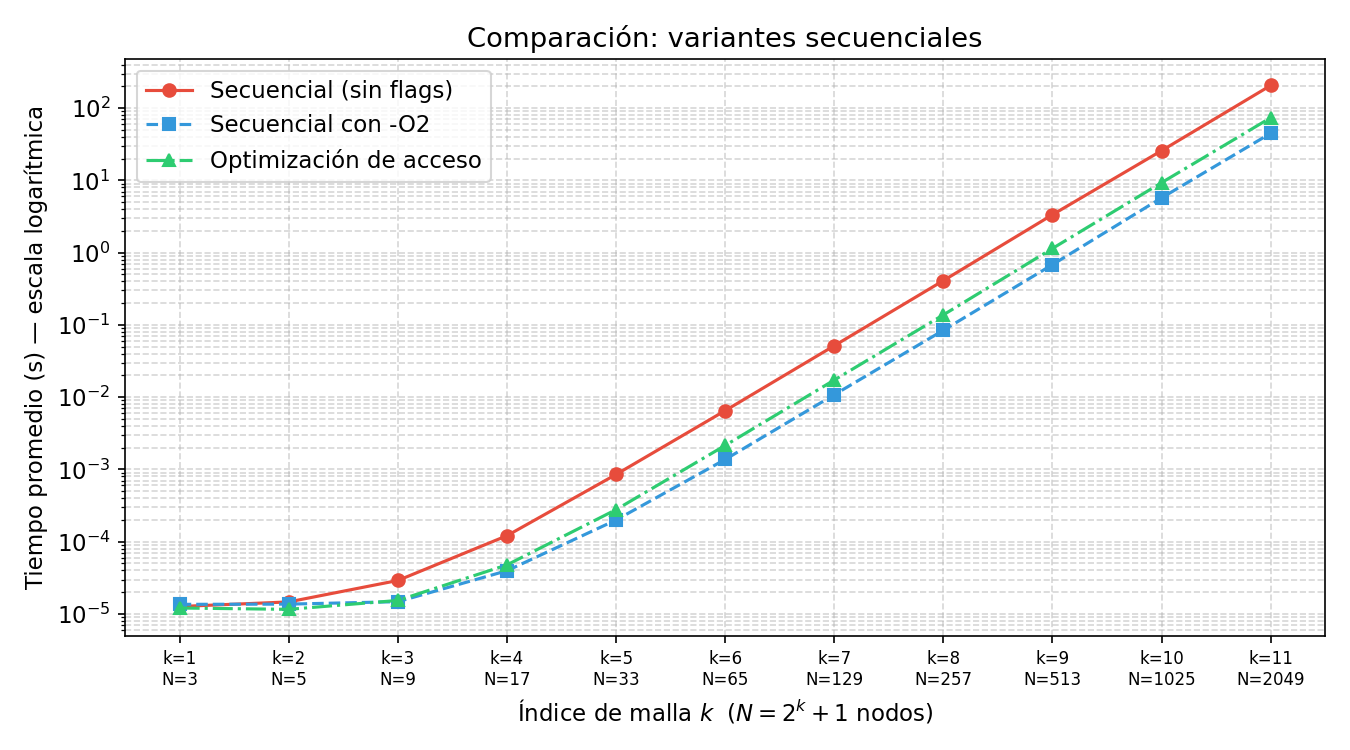
\includegraphics[width=0.9\textwidth]{charts/comparacion_secuencial.png}
  \caption{Comparación de tiempos de ejecución de las tres variantes secuenciales en escala logarítmica. La variante con \texttt{-O2} es la más rápida, seguida de la optimización manual de memoria, y finalmente el secuencial base.}
  \label{fig:comp_sec}
\end{figure}

\begin{figure}[H]
  \centering
  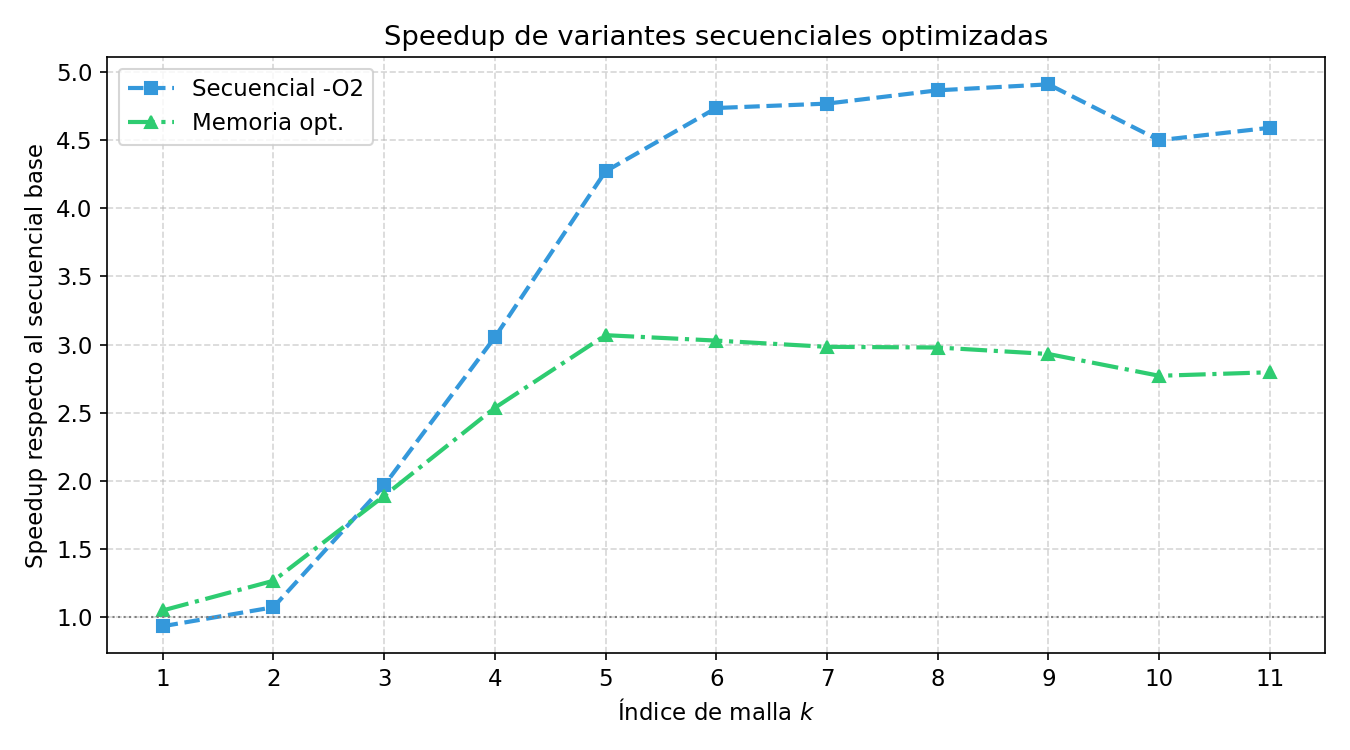
\includegraphics[width=0.9\textwidth]{charts/speedup_secuencial.png}
  \caption{Speedup de las variantes optimizadas respecto al secuencial base. La optimización por compilador (\texttt{-O2}) alcanza $\approx 4.9\times$ para mallas grandes; la optimización manual de memoria converge a $\approx 2.8\times$.}
  \label{fig:speedup_sec}
\end{figure}

\begin{figure}[H]
  \centering
  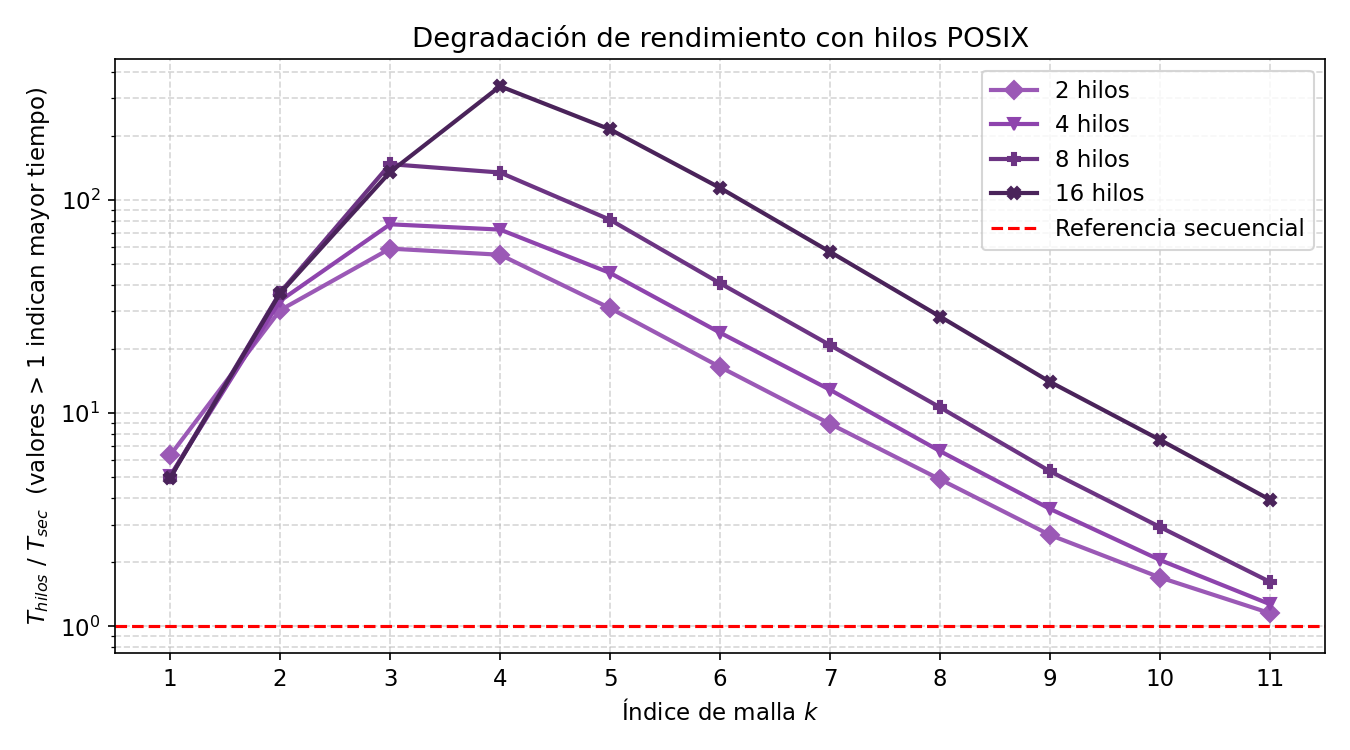
\includegraphics[width=0.9\textwidth]{charts/ratio_hilos.png}
  \caption{Razón $T_{\text{hilos}} / T_{\text{sec}}$ en escala logarítmica. Valores superiores a 1 (línea roja) indican que los hilos son más lentos que el secuencial. La degradación es más pronunciada para $k$ pequeños y empeora con más hilos.}
  \label{fig:ratio_hilos}
\end{figure}

\begin{figure}[H]
  \centering
  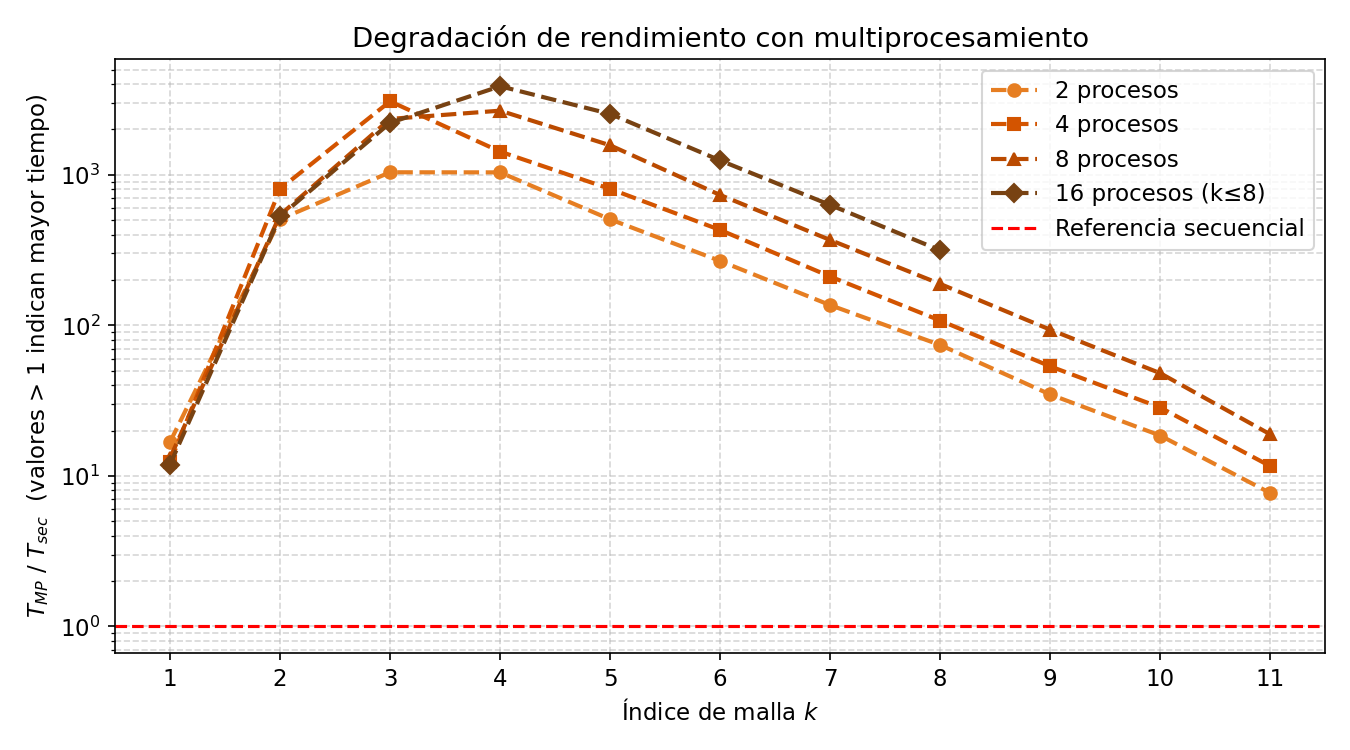
\includegraphics[width=0.9\textwidth]{charts/ratio_procesos.png}
  \caption{Razón $T_{\text{MP}} / T_{\text{sec}}$ para las variantes de multiprocesamiento. Los procesos son entre 10 y 30$\times$ más lentos que el secuencial para mallas medianas ($k=6..8$).}
  \label{fig:ratio_proc}
\end{figure}

\begin{figure}[H]
  \centering
  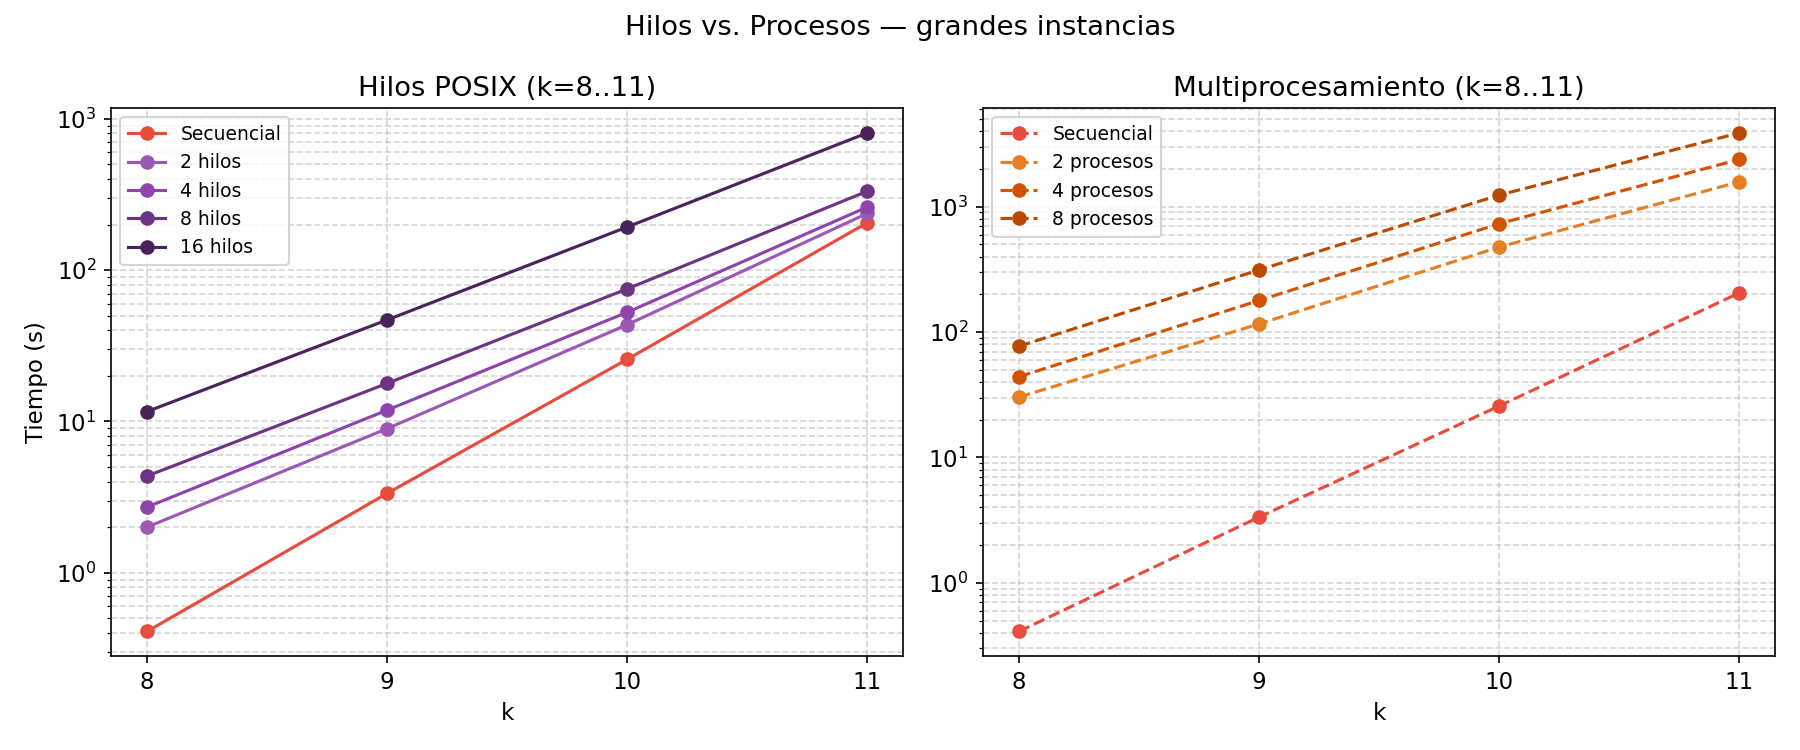
\includegraphics[width=\textwidth]{charts/hilos_vs_procesos.png}
  \caption{Comparación directa de hilos y procesos para mallas grandes ($k=8..11$). Los hilos alcanzan tiempos comparables al secuencial para $k=11$, mientras que los procesos permanecen órdenes de magnitud por encima.}
  \label{fig:hilvsproc}
\end{figure}

\begin{figure}[H]
  \centering
  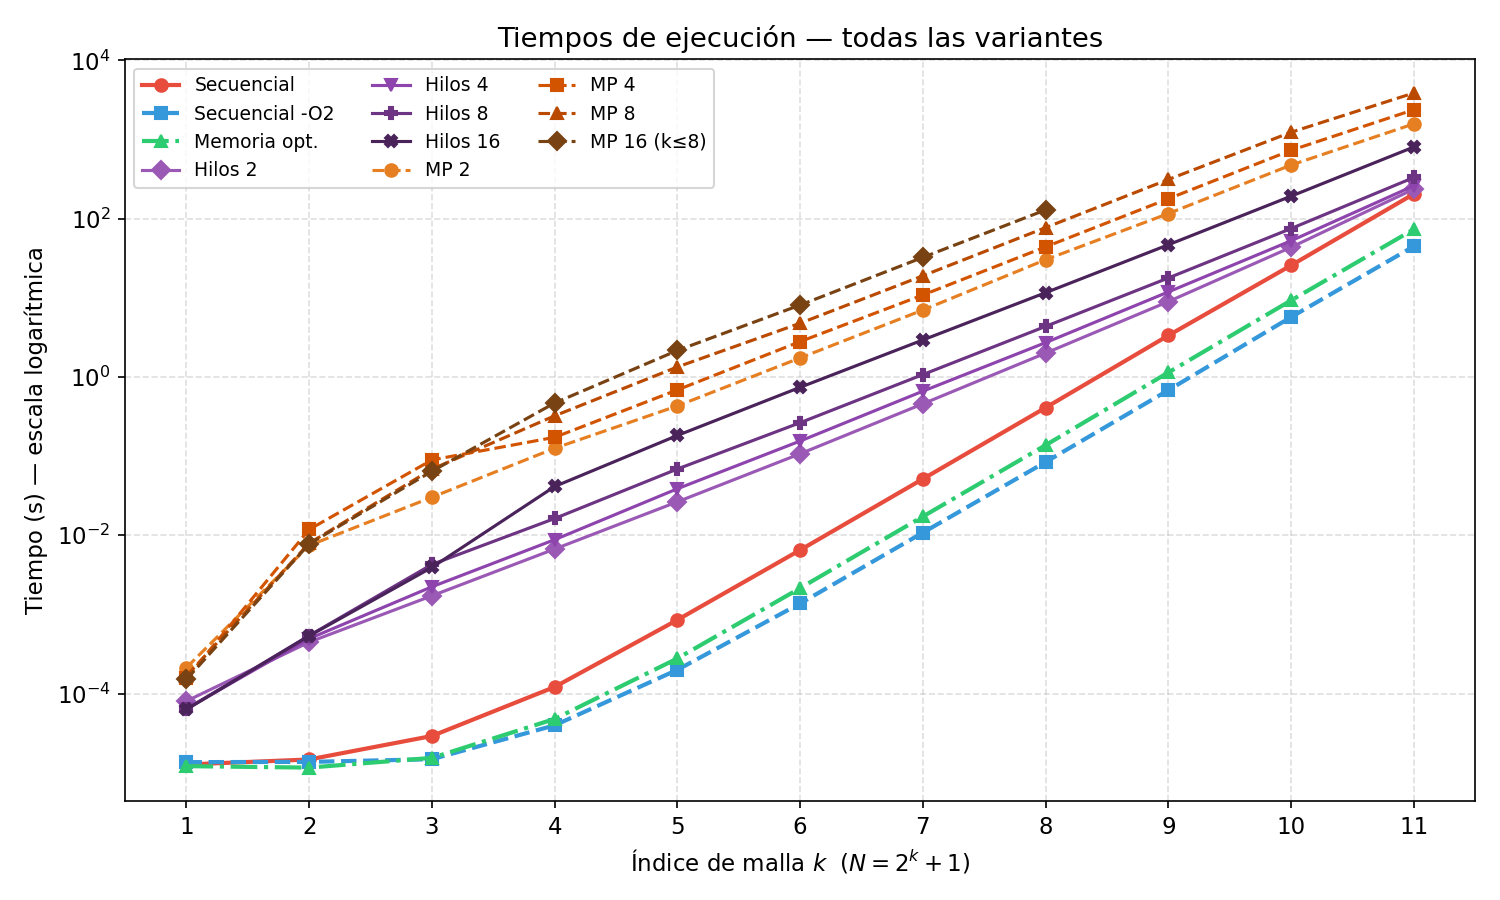
\includegraphics[width=0.9\textwidth]{charts/tiempo_ejecucion.png}
  \caption{Tiempos de ejecución de todas las variantes en escala logarítmica. Las variantes secuenciales optimizadas dominan la zona inferior; los hilos se agrupan cerca de la referencia secuencial para mallas grandes; los procesos son ampliamente más costosos.}
  \label{fig:tiempo_all}
\end{figure}

% ─────────────────────────────────────────────────────────────────────────────
\section{Análisis de resultados}

\subsection{Optimizaciones de compilador (\texttt{-O2})}

La bandera \texttt{-O2} es la intervención de mayor impacto: reduce el tiempo de
ejecución en un factor $4.5$--$4.9\times$ para mallas de $k \geq 7$ (véase
Tabla~\ref{tab:secuencial_flag} y Figura~\ref{fig:speedup_sec}).  Para $k \leq 2$
($N \leq 5$ nodos), el speedup cae a $\approx 1$ porque el tiempo de
inicialización y llamadas al sistema domina sobre el cómputo numérico.  Para $k=3$
el speedup es $\approx 2$, y se estabiliza alrededor de $4.8\times$ para $k \geq 6$.

Este comportamiento refleja el efecto del \emph{loop unrolling} y la
vectorización automática que \texttt{-O2} aplica al lazo de Jacobi.  Con $N$ grande,
el lazo interno (\texttt{for j = 1; j < N-1; j++}) se ejecuta millones de veces
y los beneficios de las instrucciones SIMD del i5-10300H (SSE4.2, AVX2) se
manifiestan plenamente.

\subsection{Optimización manual de memoria}

La variante \texttt{JacobiMemory} obtiene un speedup de $\approx 2.8\times$ para
mallas grandes, aproximadamente la mitad del beneficio de \texttt{-O2}.  Sus
cuatro optimizaciones tienen efectos distintos:

\begin{enumerate}
  \item \textbf{Fusión del lazo de barrido y residuo}: elimina una pasada
    completa sobre el vector por iteración, reduciendo el tráfico de memoria.
  \item \textbf{Swap de punteros}: evita copiar $N$ doubles en cada iteración
    ($\mathcal{O}(N)$ operaciones → $\mathcal{O}(1)$).
  \item \textbf{Verificación infrecuente}: reducir las verificaciones de
    convergencia de cada iteración a cada 50 no modifica la solución final
    (el RMS se reduce monótonamente) pero ahorra $\approx 98\%$ de los cómputos
    del residuo.
  \item \textbf{Aritmética de punteros}: mejora marginalmente la localidad de
    acceso en la caché L1.
\end{enumerate}

El speedup es consistente ($2.77$--$3.07$) para $k \geq 5$, ligeramente inferior
para $k$ pequeños donde la latencia de inicialización es comparable al cómputo.
Un outlier notable: en la primera corrida de $k=10$, \texttt{memory} tardó
10.65~s frente a $\approx 9.1$~s en las corridas restantes, probablemente por un
fallo de página masivo (\emph{page fault}) en la primera asignación de memoria
del proceso.

\subsection{Paralelismo con hilos: el costo de la barrera}

El resultado más sorprendente es que \textbf{todos los hilos son más lentos que la
versión secuencial} en todos los tamaños de malla probados.  El speedup máximo
observado es apenas $0.868$ (con 2 hilos para $k=11$), lo que significa que 2
hilos tardan un 15\% más que 1 hilo.

La explicación fundamental reside en la estructura del método de Jacobi con
barreras~\cite{burkardt}:

\begin{itemize}
  \item Para $k=11$ ($N=2\,049$), el método requiere $\approx 12.7$ millones de
    iteraciones.  Con $p$ hilos, cada iteración contiene exactamente una
    llamada a \texttt{pthread\_barrier\_wait} por hilo.  En total, hay
    $12.7 \times 10^6 \times p$ invocaciones de barrera durante la ejecución.
  \item Cada invocación de barrera tiene un costo fijo (incluso si es mínimo,
    $\approx 100$~ns en Linux), multiplicado por millones implica segundos de
    overhead acumulado.
  \item El trabajo útil por iteración por hilo es $\approx (N-2)/p$ sumas y
    multiplicaciones.  Para $k=7$ ($N=129$) con 16 hilos, cada hilo procesa
    solo $\approx 8$ nodos por barrido.  El overhead de la barrera eclipsa
    completamente el cómputo.
\end{itemize}

Pese a ello, se observa una mejora relativa conforme crece $k$: el speedup de 2
hilos mejora de $0.017$ en $k=3$ a $0.868$ en $k=11$.  Esto confirma que el
problema requeriría mallas mucho más grandes ($k \geq 13$ o más) para que los
hilos sean competitivos con el secuencial.

\subsection{Paralelismo con procesos: overhead masivo}

Las variantes de multiprocesamiento muestran tiempos hasta \textbf{4 órdenes de
magnitud} mayores que el secuencial para mallas pequeñas ($k=2$, ratio $\approx
500\times$).  Para $k=11$ con 2 procesos, el ratio es $\approx 7.7\times$
(1580~s~MP frente a 205~s secuencial).

El overhead proviene de múltiples fuentes:
\begin{itemize}
  \item \textbf{Creación de procesos con \texttt{fork()}}: aunque es una sola
    llamada al inicio, el kernel debe clonar las tablas de páginas y los
    descriptores de archivos.
  \item \textbf{Acceso a memoria compartida}: cada proceso accede al vector $u$
    a través de la región \texttt{mmap}, que requiere TLB entries adicionales y
    puede generar fallos de caché cruzados entre núcleos.
  \item \textbf{Sincronización implícita}: la implementación actual no usa
    barreras explícitas entre iteraciones; esto puede generar lecturas de datos
    parcialmente actualizados, afectando la convergencia o produciendo condiciones
    de carrera.
  \item \textbf{Scheduling del SO}: el planificador del kernel puede desalojar
    procesos entre iteraciones, introduciendo latencias variables.
\end{itemize}

Un hecho notable es que \emph{más procesos no siempre implica peor rendimiento}
para mallas grandes: para $k=11$, mp2 tardó 1580~s mientras que mp4 tardó
2383~s y mp8 tardó 3877~s.  Esto sugiere que la contención en el acceso a la
región compartida escala con el número de procesos.

\subsection{Comparación global de variantes}

La Tabla~\ref{tab:resumen} resume los tiempos promedio para $k=11$ ($N=2\,049$,
el caso de mayor carga):

\begin{table}[H]
\centering
\begin{tabular}{lrr}
\toprule
\textbf{Variante} & \textbf{Tiempo (s)} & \textbf{Speedup vs.\ sec} \\
\midrule
Secuencial base        & 205.57 & 1.000 \\
Secuencial -O2         &  44.79 & 4.590 \\
Optimización memoria   &  73.50 & 2.797 \\
Hilos 2                & 236.81 & 0.868 \\
Hilos 4                & 260.81 & 0.788 \\
Hilos 8                & 331.89 & 0.619 \\
Hilos 16               & 805.70 & 0.255 \\
Multiprocesamiento 2   & 1580.12 & 0.130 \\
Multiprocesamiento 4   & 2382.76 & 0.086 \\
Multiprocesamiento 8   & 3877.12 & 0.053 \\
\bottomrule
\end{tabular}
\caption{Resumen de rendimiento para $k=11$ ($N=2\,049$). El orden de mérito es: \texttt{-O2} $>$ \texttt{memory} $>$ secuencial base $>$ hilos~2 $>$ \ldots $>$ MP~8.}
\label{tab:resumen}
\end{table}

El ranking es claro: la optimización de compilador supera a todas las demás
estrategias para este problema.  La optimización manual de memoria ocupa el
segundo lugar.  Todos los esquemas paralelos son contraproducentes.

% ─────────────────────────────────────────────────────────────────────────────
\section{Conclusiones}

\begin{enumerate}

  \item \textbf{La optimización del compilador (\texttt{-O2}) es la estrategia
    más eficaz} para el método de Jacobi 1D: ofrece un speedup de $\approx 4.9\times$
    con cero esfuerzo de programación.  Para aplicaciones reales, compilar con
    \texttt{-O2} o \texttt{-O3} debe ser el primer paso antes de cualquier
    optimización manual o paralela.

  \item \textbf{La optimización manual de acceso a memoria logra $\approx 2.8\times$},
    casi la mitad del beneficio de \texttt{-O2}.  La técnica más impactante es
    la verificación infrecuente del residuo (cada 50 iteraciones), seguida de
    la eliminación de la copia de arrays mediante swap de punteros.  Estas
    técnicas son portables y no dependen del compilador.

  \item \textbf{Los hilos POSIX son contraproducentes} para el método de Jacobi
    1D en todas las mallas probadas ($N \leq 2\,049$).  El overhead de la barrera
    de sincronización por iteración supera el trabajo útil repartido entre hilos.
    El speedup mejora con el tamaño de la malla ($0.017$ para $k=3$ hasta $0.868$
    para $k=11$ con 2 hilos), lo que sugiere que mallas mayores ($k \geq 14$ o
    más) podrían compensar el overhead.

  \item \textbf{El multiprocesamiento es aún peor que los hilos}: los tiempos son
    entre 2 y 4 órdenes de magnitud mayores que el secuencial.  El overhead de
    \texttt{fork()}, la latencia de la memoria compartida y la falta de sincronización
    explícita entre iteraciones hacen que esta estrategia sea inadecuada para
    problemas 1D de pocas decenas o centenas de nodos.

  \item \textbf{Lección de diseño}: el paralelismo solo compensa cuando hay
    suficiente trabajo útil por unidad de sincronización.  Para el método de
    Jacobi 1D, la granularidad del problema es demasiado fina.  En contraste,
    problemas 2D o 3D con mallas grandes tendrían una relación trabajo/sincronización
    mucho más favorable, y el paralelismo podría entonces ofrecer speedups
    positivos.

  \item \textbf{Impacto del hardware}: el i5-10300H tiene solo 4 núcleos físicos.
    Más allá de 4 hilos lógicos se activa el Hyper-Threading, que comparte
    recursos de caché L1/L2, amplificando el efecto negativo de las barreras
    y explicando el colapso de rendimiento observado con 8 y 16 hilos.

\end{enumerate}

% ─────────────────────────────────────────────────────────────────────────────
\section{Bibliografía}

\begin{thebibliography}{9}

\bibitem{burkardt}
  Burkardt, J. (2014).
  \textit{Jacobi Iterative Solution of Poisson's Equation in 1D}.
  Departamento de Ciencias Computacionales, Florida State University.
  Disponible en \texttt{docs/reference/jacobi\_poisson\_1d.pdf}.

\bibitem{amdahl}
  Amdahl, G.~M. (1967).
  Validity of the single-processor approach to achieving large scale
  computing capabilities.
  \textit{AFIPS Conference Proceedings}, 30, 483--485.

\bibitem{lopez2017}
  López, R. (2017).
  \textit{Introducción a la computación de alto rendimiento}.
  Notas de cátedra.

\bibitem{ferestrepoca}
  Ferestrepoca, J. (2019).
  \textit{Computación Paralela: fundamentos y aplicaciones}.
  Universidad Nacional de Colombia.

\bibitem{montero2011}
  Montero, F. \& Antunez, M. (2011).
  \textit{Sistemas Operativos: hilos y procesos}.
  Apuntes de clase, Universidad Politécnica de Madrid.

\bibitem{intel_i5}
  Intel Corporation (2020).
  \textit{Intel Core i5-10300H Processor Specifications}.
  \url{https://www.intel.com/content/www/us/en/products/sku/201897/intel-core-i5-10300h-processor-8m-cache-up-to-4-50-ghz/specifications.html}

\end{thebibliography}

\end{document}
